\documentclass[10pt]{article}
\setlength{\textwidth}{6.3in}
\setlength{\textheight}{9in}
\setlength{\oddsidemargin}{0in}
\setlength{\evensidemargin}{0in}
\setlength{\topmargin}{-.5in}
%\parindent=0in
\linespread{1.3}
\usepackage{ mathrsfs }
\usepackage{amsthm}
\usepackage{ amssymb }
\usepackage{graphicx}
\newtheorem{theorem}{Theorem}[section]
\newtheorem{lemma}[theorem]{Lemma}

\usepackage{amsmath}
\usepackage{amsfonts}
\usepackage{fancyhdr}
\usepackage{nicematrix}
\usepackage{tikz}

\pagestyle{fancy}
\headheight = 14.5pt
\lhead{Exam 1 Practice, Thomas Zeng }
\rhead{CS 254, Winter 2023}
\cfoot{\thepage}

\begin{document}

\noindent
This is a practice exam that covers a proper subset of the information you are expected to know for the actual exam. Please use it as a tool to both practice concepts we've learned so far and also to gauge your comfort with these concepts.\\

\noindent
\textbf{Disclaimer: }This is \textbf{just} a practice exam and is meant to be done for review purposes. It is in no way an indicator of the actual exam in difficulty or content (as I am not Anna and do not have access to the actual exam).

\newpage
\noindent
\textbf{A.} Consider the ``suffix'' operation over languages $A$ and $B$:
\[A\text{ suffix } B=\{w|w\in A \text{ and some suffix of }w\in B \}.\]
A string $x$ is a suffix of a string $w$ if there exists a string $y$ such that $yx=w.$ Show that regular languages are closed under the suffix operation
(\textit{This is a variation of problem 2 on Problem Set 3}).\\

\noindent
\textbf{Answer:}

\begin{proof}
    % proof has problems with the alphabhet used



    Let $A$ and $B$ be regular languages.
    WLOG, assume $A$ and $B$ have the same alphabet\footnote{As if they do not, we can construct languages $A',B'$ that accept the same strings as $A,B$ but use the union of the alphabets of $A$ and $B$ as their alphabet.} which we denote $\Sigma$.
    We next define the languages
    \[C =\{w|w\in A\}\]
    and
    \[D=\{w|w\in\Sigma^*\text{ and some suffix of }w\in B\}.\]
    By the definition of suffix, we have $A\text{ suffix }B=C\cap D.$ Thus, to show $A\text{ suffix } B$ is regular, it suffices to show that $C,D$ are regular.
    
    We first show $C$ is regular. By our definition of $C,$ we have $C=A.$ As $A$ is regular, therefore $C$ is regular.
    
    We next show $D$ is regular. As $B$ is regular there exists some NFA $M=(Q,\Sigma,\delta,q_0,F)$ where $L(M)=B.$
    % Therefore, there exists DFA $M,N$ s.t. $L(M)=A$ and $L(N)=B.$ We denote $N=(Q,\Sigma,\delta,q_0,F).$
    We now construct an NFA $N=(Q_D,\Sigma_D,\delta_D,q_{0_D},F_D)$ where:
    \begin{align*}
        Q_D &= Q \cup q_{0_D}\\
        \Sigma_D &= \Sigma\\
        \delta_D(q,w)&=\begin{cases}
            \delta(q,w),\quad& q\neq q_{0_D}\\
            \{q_0, q_{0_D}\} ,\quad& q= q_{0_D}
        \end{cases}\quad\text{ where }q\in Q_D,\;
         w\in\Sigma_D\cup\epsilon\\
        q_{0_D} &= q_{0_D}\quad\text{(the start state is a new state)}\\
        F_D &= F.
    \end{align*}
    We assert that $L(N)=D$ as it adds a new state $q_{0_D}$ that nondeterministicaly branches to test if each suffix of the input string is in $B$.
    Therefore $D$ is regular. And thus $A\text{ suffix } B$ is regular.
\end{proof}

\newpage

\noindent
\textbf{B.} For languages $A$ and $B$, let the ``shuffle'' of $A$ and $B$ be the language
\[\{w|w=a_1b_1...a_kb_k,\text{ where }a_1...a_k\in A\text{ and }b_1...b_k\in B, \text{ each }a_i,b_i\in\Sigma^*\}.\]
Show that the class of regular languages is closed under shuffle (\textit{This is problem 1.42 in Sipser}).\\

\noindent
\textbf{Answer:}

\begin{proof}
    Let $A,B$ be regular. Let $M = (Q_A,\Sigma,\delta_A,q_{0_A}, F_A)$ and $N = (Q_B,\Sigma,\delta_B,q_{0_B}, F_B)$ where $L(M)=A$ and $L(N)=B.$ Let $C$ be the shuffle of $A$ and $B.$

    We now construct a NFA $O = (Q_C,\Sigma,\delta_C,q_{0_C}, F_C)$ where
    \begin{align*}
        Q_C &= Q_A \times Q_B \\
        \Sigma &= \Sigma\\
        \delta_C((q_a\, q_b),w)&= \{ (\delta_A(q_a, w), q_b), (q_a, \delta_B(q_b, w)\}
\\%\quad\text{ where }q\in Q_D,\;
        q_{0_C} &= (q_{0_A}, q_{0_B})\\
        F_C &= F_A\times F_B.%\{(q_a, q_b)| q_a\in F_A \text{ and }q_b\in F_B\}.
    \end{align*}
    We assert that $L(O)=C$ as $O$ nondeterministicaly checks whether each letter is part of a string in $A$ versus $B$ by simulating it on its respective dfa. Therefore the shuffle operation is closed.
\end{proof}

\newpage

\noindent
\textbf{C.} Prove the following languages are irregular using the pumping lemma.\\
\textbf{C.A} Let $L=\{w|w=0^i1^j0^k \text{ where } i+k=j \text{ and }i>0\}.$\\
\textbf{C.B} Let $L=\{w|w\in\{\text{``(''}, \text{``)''}\}^* \text{ is a valid nesting of parentheses}\}$ e.g. $(())()\in L$ but $((()\notin L.$\\
\textbf{C.C} Let $L=\{w|w=(ab)^nb^k \text{ where }k>n>0\}$.\\
\textbf{C.D} Let $L=\{w|w=a^{n^3} \text{ where }n>0 \text{ and is an integer}\}$.\\


\noindent
\textbf{Answer:}
The typical structure for showing a language $L$ is not regular is to use the Pumping Lemma with the following structure:

\begin{proof}
    Assume $L$ is regular. So there is a pumping length $p > 0$ for $L.$ Now consider the string
    \begin{equation}\label{eq:string}
        w= \text{XXXXX}.
    \end{equation}
    Note that $w\in L$ and $|w|\ge p.$ By condition three of the PL, $w$ can be decomposed into the string $xyz$ where
    \begin{equation} \label{eq:xy}
        xy \text{ must be XXXXX.}
    \end{equation}
    By condition two of the PL,
    \begin{equation} \label{eq:y}
        y \text{ must XXXXX.}
    \end{equation}
    Now lets consider
    \begin{equation} \label{eq:i}
        i =\text{XXXXX.}
    \end{equation}
    We thus have
    \begin{equation} \label{eq:xyiz}
        xy^iz=\text{XXXXX}\notin L.
    \end{equation}
    This is a contradiction and therefore $L$ is not regular.
\end{proof}

% \noindent
% Therefore we can answer each Pumping Lemma question by filling this structure in.\\

\noindent
\textbf{C.A}\\


\noindent
\eqref{eq:string} $w=0^p1^p$\\
\eqref{eq:xy} in the string $0^p$\\
\eqref{eq:y} be of the form $0^k$ for some $0<k\le p$\\
\eqref{eq:i} $0$\\
\eqref{eq:xyiz} $0^{p-k}1^p$\\

\noindent
\textbf{C.B}\\

\noindent
\eqref{eq:string} $w=(^p)^p$\\
\eqref{eq:xy} in the string $(^p$\\
\eqref{eq:y} be of the form $(^k$ for some $0<k\le p$\\
\eqref{eq:i} $0$\\
\eqref{eq:xyiz} $(^{p-k})^p$\\

\noindent
\textbf{C.C}\\

\noindent
\eqref{eq:string} $w=(ab)^pb^{p+1}$\\
\eqref{eq:xy} in the string $(ab)^p$\\
\eqref{eq:y} be of the form $(ab)^k$ for some $0<k\le p$ or of the form $b(ab)^*a,(ab)^*a, b(ab)^*$\\
\eqref{eq:i} $2$\\
\eqref{eq:xyiz} In the first case we have $(ab)^{p+k}b^{p+1}$ which is not in the language. In the second case we would have a string \textbf{not} of the form $(ab)^*b^*$ so it is also not in the language\\

\noindent
\textbf{C.D}\\

\noindent
\eqref{eq:string} $w=a^{p^3}$\\
\eqref{eq:xy} in the string $a^p$\\
\eqref{eq:y} be of the form $a^k$ for some $0<k\le p$\\
\eqref{eq:i} $2$\\
\eqref{eq:xyiz} $a^{p^3+k}.$ This is true as $p^3<p^3+k\le p^3+p<(p+1)^3$ so $p^3+k$ is not the cubic of some integer.\\

\newpage

\noindent
\textbf{D.} In the previous question, we showed the language of valid nestings of parentheses i.e. $$L=\{w|w\in\{\text{``(''}, \text{``)''}\}^* \text{ is a valid nesting of parentheses}\}$$ is not regular. However, it is context free.\\
\textbf{D.A} Construct a Context Free Grammar for this language.\\

\noindent
\textbf{Answer:}\\
\begin{align*}
    S &\to P\\
    P &\to PP|(P)|\epsilon
\end{align*}\\


\noindent
\textbf{D.B} Use your grammar to generate a parse tree for the string ``(()())()''.\\


\noindent
\textbf{Answer:}

\begin{center}
    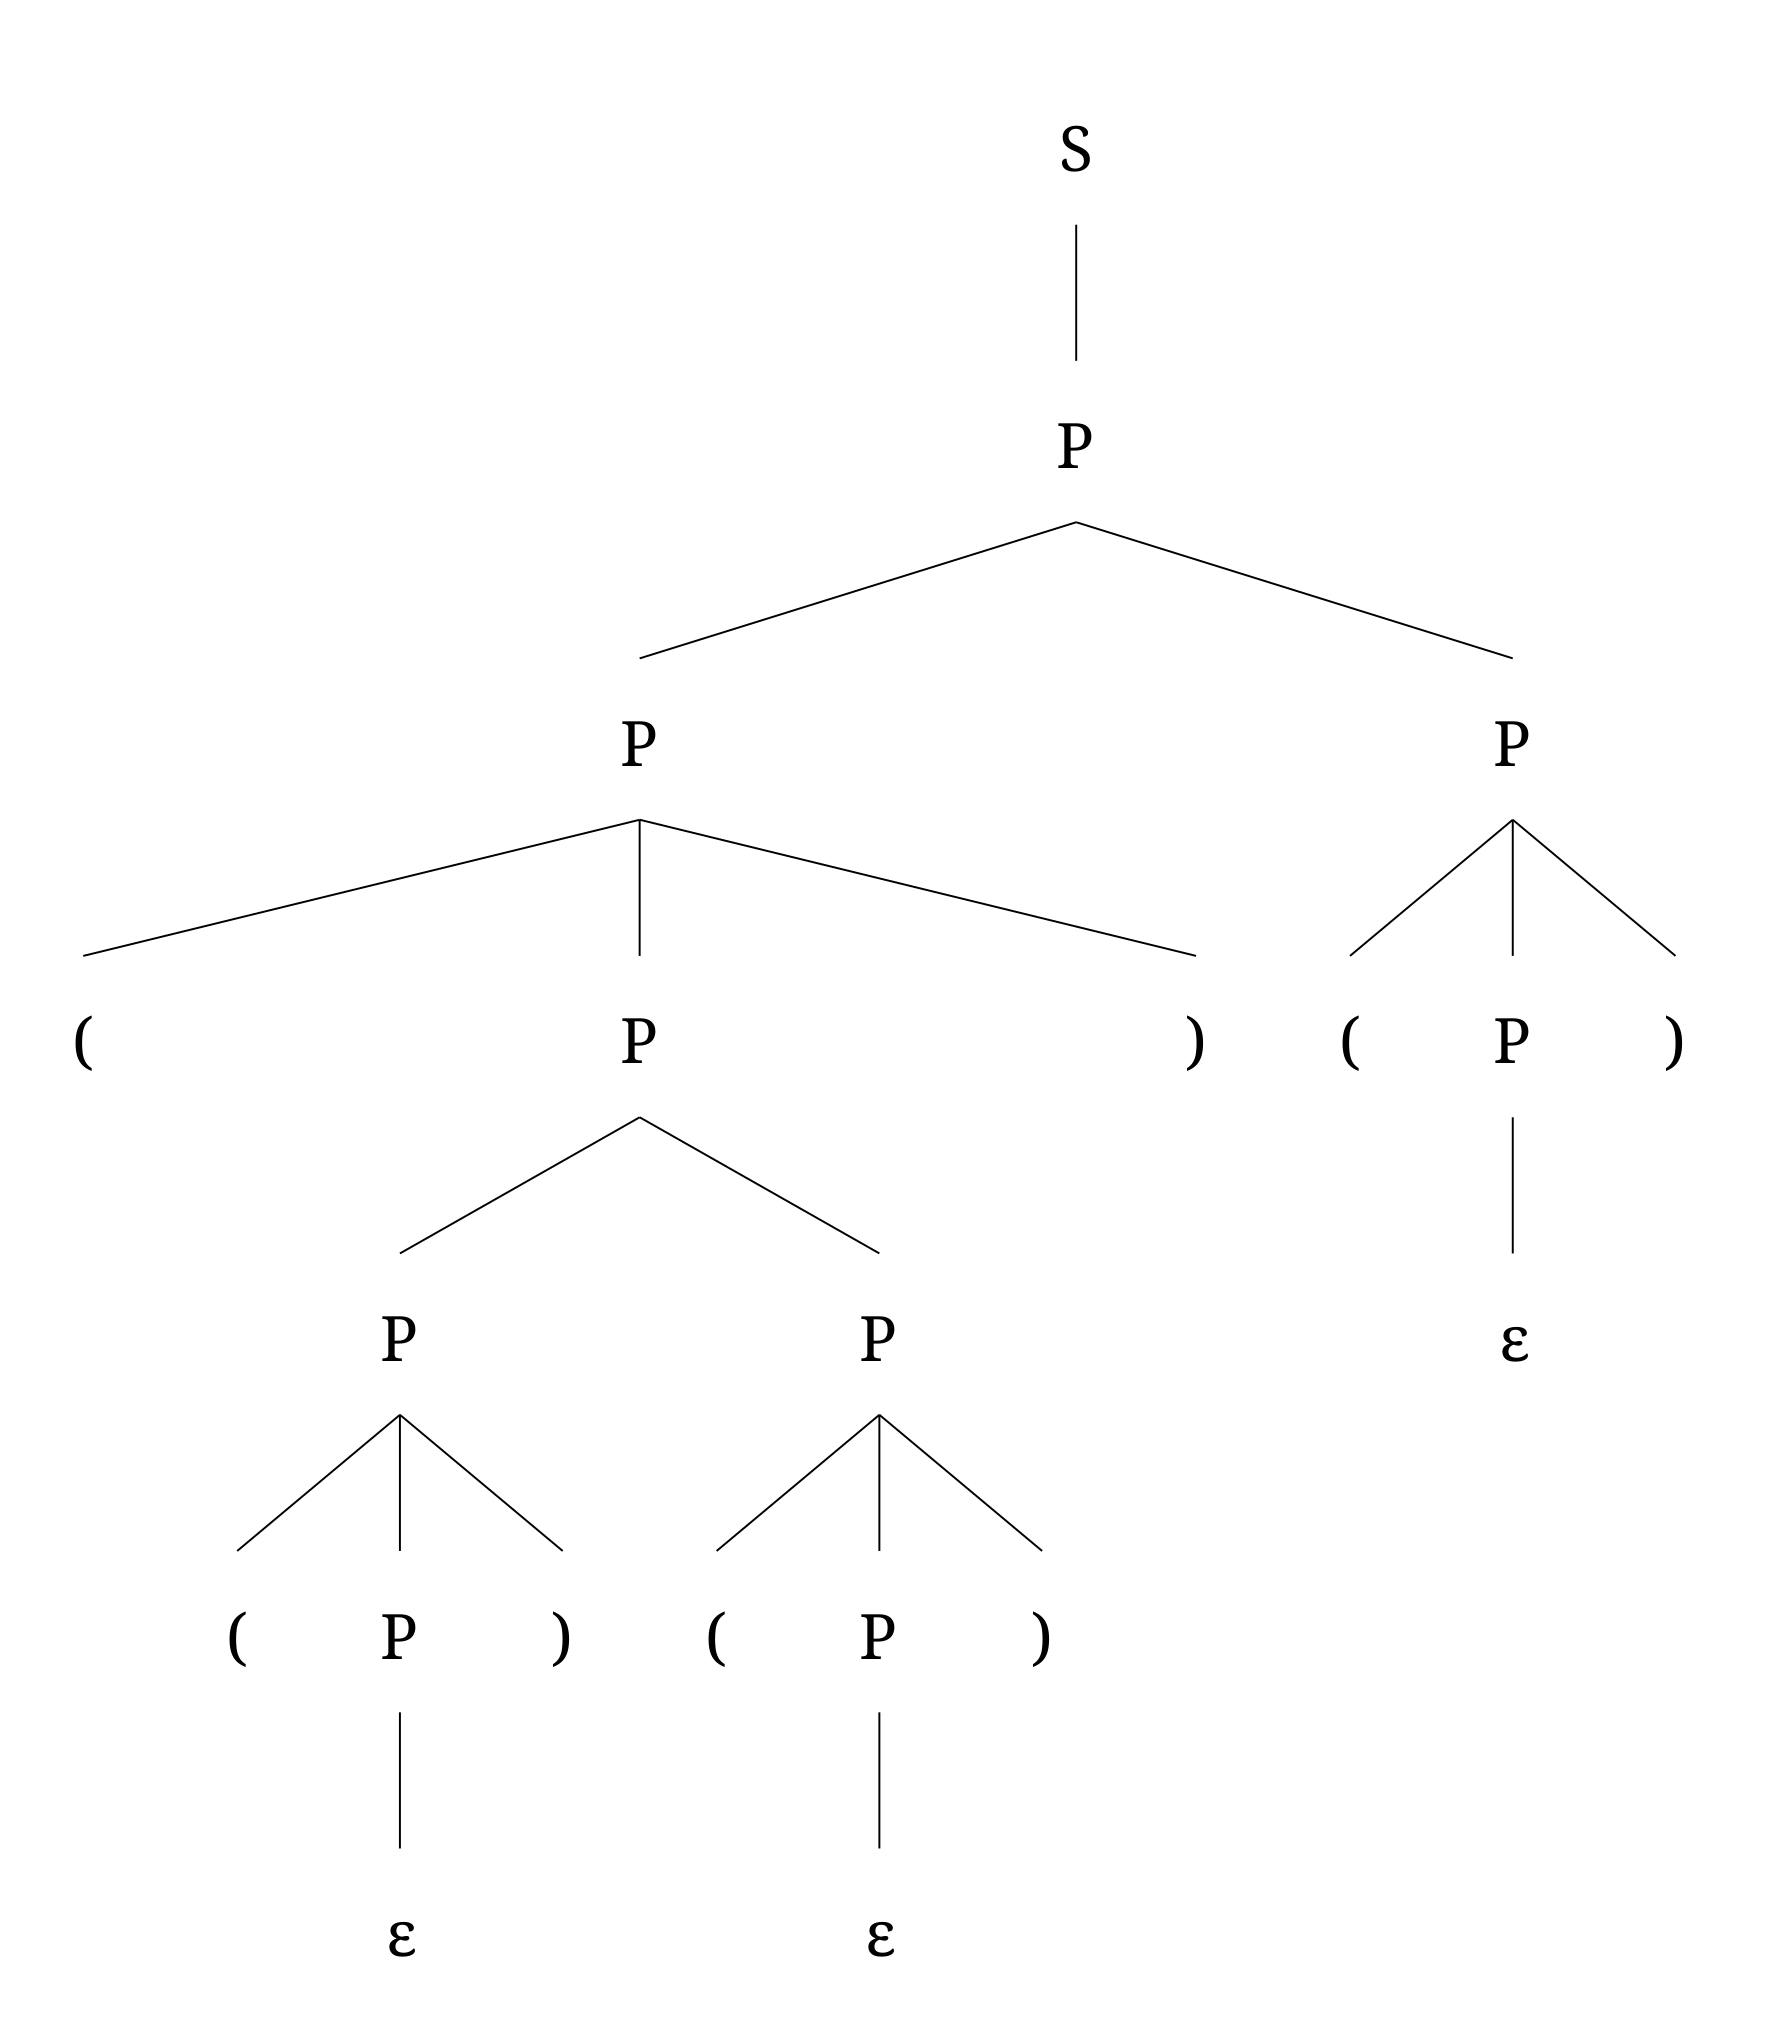
\includegraphics[width=0.5\textwidth]{parse_tree.png}
\end{center}

\noindent
\textbf{D.C} Construct a PDA for this language.\\

\noindent
\textbf{Answer:}


\begin{center}
    \begin{tikzpicture}[scale=0.2]
    \tikzstyle{every node}+=[inner sep=0pt]
    \draw [black] (22.1,-25.3) circle (3);
    \draw (22.1,-25.3) node {$q_0$};
    \draw [black] (37.8,-25.3) circle (3);
    \draw (37.8,-25.3) node {$q_1$};
    \draw [black] (53.7,-25.3) circle (3);
    \draw (53.7,-25.3) node {$q_2$};
    \draw [black] (53.7,-25.3) circle (2.4);
    % \draw [black] (11.9,-25.3) circle (3);
    % \draw (11.9,-25.3) node {$qq$};
    \draw [black] (25.1,-25.3) -- (34.8,-25.3);
    \fill [black] (34.8,-25.3) -- (34,-24.8) -- (34,-25.8);
    \draw (29.95,-25.8) node [below] {$\epsilon,\epsilon\to S\$$};
    \draw [black] (40.8,-25.3) -- (50.7,-25.3);
    \fill [black] (50.7,-25.3) -- (49.9,-24.8) -- (49.9,-25.8);
    \draw (45.75,-25.8) node [below] {$\epsilon,\$\to\epsilon$};
    \draw [black] (36.477,-22.62) arc (234:-54:2.25);
    \draw (37.8,-18.05) node [label={[label distance=1.2cm] $\epsilon,P\to \epsilon$}] {};
    \draw (37.8,-18.05) node [label={[label distance=0.8cm] $\epsilon,P\to )P($}] {};
    \draw (37.8,-18.05) node [label={[label distance=0.4cm] $\epsilon,P\to PP$}] {};
    \draw (37.8,-18.05) node [above] {$\epsilon,S\to P$};
    \fill [black] (39.12,-22.62) -- (40,-22.27) -- (39.19,-21.68);
    \draw [black] (14.9,-25.3) -- (19.1,-25.3);
    \fill [black] (19.1,-25.3) -- (18.3,-24.8) -- (18.3,-25.8);
    
    \draw [black] (39.123,-27.98) arc (54:-234:2.25);
    \draw (37.8,-32.55) node [below] {$(,(\to\epsilon$};
    \draw (37.8,-32.55) node [label={[label distance=-0.8cm] $),)\to\epsilon$}] {};
    
    \fill [black] (36.48,-27.98) -- (35.6,-28.33) -- (36.41,-28.92);
    
    
    \end{tikzpicture}
    \end{center}

    \noindent
    \textbf{D.D} Consider the language
    \[L' = \{(^i)^j|0<i<j\}\]
    which is context free. Construct a CFG for this language.\\

    \noindent
    \textbf{Answer:}

    \begin{align*}
        S&\to (P)\\
        P &\to (P)|C)\\
        C &\to C)|\epsilon\\
    \end{align*}

    \noindent
    \textbf{D.E} Construct the grammar for the language $L\circ L'.$\\
    
    \noindent
    \textbf{Answer:}
    
    \begin{align*}
        S &\to S_0S_1\\
        S_0 &\to P_0\\
        P_0 &\to P_0P_0|(P_0)|\epsilon\\
        S_1&\to (P_1)\\
        P_1 &\to (P_1)|C_1)\\
        C_1 &\to C_1)|\epsilon
    \end{align*}


    \newpage
    \noindent
    \textbf{E} In an alien world far away, phone numbers are of the form \texttt{04xy}, where \texttt{x} represents any digit in the set $\{7,9\}$ and \texttt{y} is either the string $11$ or $84.$\\

    \noindent
    \textbf{E.A}  Write a textbook regular expression that matches exactly these strings over the $\Sigma=\{0,1,...,9\}.$\\
    
    \noindent
    \textbf{Answer:}\\
    $04(7\cup9)(11\cup84)$\\

    \noindent
    \textbf{E.B}  Convert this regular expression into a NFA using the algorithm from Sipser.\\

    \noindent
    \textbf{Answer:}\\

    \begin{center}
        \begin{tikzpicture}[scale=0.2]
        \tikzstyle{every node}+=[inner sep=0pt]
        \draw [black] (18.5,-7.6) circle (3);
        \draw (18.5,-7.6) node {$q_1$};
        \draw [black] (8,-16.3) circle (3);
        \draw (8,-16.3) node {$q_2$};
        \draw [black] (18.5,-16.3) circle (3);
        \draw (18.5,-16.3) node {$q_3$};
        \draw [black] (8,-7.6) circle (3);
        \draw (8,-7.6) node {$q_0$};
        \draw [black] (8,-24.5) circle (3);
        \draw (8,-24.5) node {$q_4$};
        \draw [black] (18.5,-24.5) circle (3);
        \draw (18.5,-24.5) node {$q_5$};
        \draw [black] (68.8,-24.5) circle (3);
        \draw (68.8,-24.5) node {$q_6$};
        \draw [black] (18.5,-33.4) circle (3);
        \draw (18.5,-33.4) node {$q_7$};
        \draw [black] (31.2,-33.4) circle (3);
        \draw (31.2,-33.4) node {$q_8$};
        \draw [black] (18.5,-43.7) circle (3);
        \draw (18.5,-43.7) node {$q_{10}$};
        \draw [black] (28.7,-43.7) circle (3);
        \draw (28.7,-43.7) node {$q_{11}$};
        \draw [black] (40,-43.7) circle (3);
        \draw (40,-43.7) node {$q_{12}$};
        \draw [black] (51.1,-43.7) circle (3);
        \draw (51.1,-43.7) node {$q_{13}$};
        \draw [black] (51.1,-43.7) circle (2.4);
        \draw [black] (18.5,-55.6) circle (3);
        \draw (18.5,-55.6) node {$q_{14}$};
        \draw [black] (28.7,-55.6) circle (3);
        \draw (28.7,-55.6) node {$q_{15}$};
        \draw [black] (40,-55.6) circle (3);
        \draw (40,-55.6) node {$q_{16}$};
        \draw [black] (51.1,-55.6) circle (3);
        \draw (51.1,-55.6) node {$q_{17}$};
        \draw [black] (51.1,-55.6) circle (2.4);
        \draw [black] (8,-43.7) circle (3);
        \draw (8,-43.7) node {$q_9$};
        \draw [black] (11,-16.3) -- (15.5,-16.3);
        \fill [black] (15.5,-16.3) -- (14.7,-15.8) -- (14.7,-16.8);
        \draw (13.25,-15.8) node [above] {$4$};
        \draw [black] (16.19,-9.51) -- (10.31,-14.39);
        \fill [black] (10.31,-14.39) -- (11.25,-14.26) -- (10.61,-13.49);
        \draw (12.3,-11.46) node [above] {$\epsilon$};
        \draw [black] (11,-7.6) -- (15.5,-7.6);
        \fill [black] (15.5,-7.6) -- (14.7,-7.1) -- (14.7,-8.1);
        \draw (13.25,-7.1) node [above] {$0$};
        \draw [black] (2.3,-7.6) -- (5,-7.6);
        \fill [black] (5,-7.6) -- (4.2,-7.1) -- (4.2,-8.1);
        \draw [black] (16.14,-18.15) -- (10.36,-22.65);
        \fill [black] (10.36,-22.65) -- (11.3,-22.56) -- (10.69,-21.77);
        \draw (12.3,-19.9) node [above] {$\epsilon$};
        \draw [black] (21.5,-24.5) -- (65.8,-24.5);
        \fill [black] (65.8,-24.5) -- (65,-24) -- (65,-25);
        \draw (43.65,-24) node [above] {$7$};
        \draw [black] (21.5,-33.4) -- (28.2,-33.4);
        \fill [black] (28.2,-33.4) -- (27.4,-32.9) -- (27.4,-33.9);
        \draw (24.85,-32.9) node [above] {$9$};
        \draw [black] (21.5,-43.7) -- (25.7,-43.7);
        \fill [black] (25.7,-43.7) -- (24.9,-43.2) -- (24.9,-44.2);
        \draw (23.6,-44.2) node [below] {$1$};
        \draw [black] (31.7,-43.7) -- (37,-43.7);
        \fill [black] (37,-43.7) -- (36.2,-43.2) -- (36.2,-44.2);
        \draw (34.35,-44.2) node [below] {$\epsilon$};
        \draw [black] (43,-43.7) -- (48.1,-43.7);
        \fill [black] (48.1,-43.7) -- (47.3,-43.2) -- (47.3,-44.2);
        \draw (45.55,-44.2) node [below] {$1$};
        \draw [black] (21.5,-55.6) -- (25.7,-55.6);
        \fill [black] (25.7,-55.6) -- (24.9,-55.1) -- (24.9,-56.1);
        \draw (23.6,-56.1) node [below] {$8$};
        \draw [black] (31.7,-55.6) -- (37,-55.6);
        \fill [black] (37,-55.6) -- (36.2,-55.1) -- (36.2,-56.1);
        \draw (34.35,-56.1) node [below] {$\epsilon$};
        \draw [black] (43,-55.6) -- (48.1,-55.6);
        \fill [black] (48.1,-55.6) -- (47.3,-55.1) -- (47.3,-56.1);
        \draw (45.55,-56.1) node [below] {$4$};
        \draw [black] (10.29,-26.44) -- (16.21,-31.46);
        \fill [black] (16.21,-31.46) -- (15.92,-30.56) -- (15.28,-31.32);
        \draw (12.3,-29.44) node [below] {$\epsilon$};
        \draw [black] (11,-24.5) -- (15.5,-24.5);
        \fill [black] (15.5,-24.5) -- (14.7,-24) -- (14.7,-25);
        \draw (13.25,-25) node [below] {$\epsilon$};
        \draw [black] (28.46,-34.62) -- (10.74,-42.48);
        \fill [black] (10.74,-42.48) -- (11.68,-42.62) -- (11.27,-41.7);
        \draw (20.52,-39.06) node [below] {$\epsilon$};
        \draw [black] (67.905,-27.363) arc (-19.63394:-125.31492:37.849);
        \fill [black] (10.38,-45.53) -- (10.74,-46.4) -- (11.32,-45.58);
        \draw (44.47,-51.28) node [below] {$\epsilon$};
        \draw [black] (11,-43.7) -- (15.5,-43.7);
        \fill [black] (15.5,-43.7) -- (14.7,-43.2) -- (14.7,-44.2);
        \draw (13.25,-44.2) node [below] {$\epsilon$};
        \draw [black] (9.98,-45.95) -- (16.52,-53.35);
        \fill [black] (16.52,-53.35) -- (16.36,-52.42) -- (15.61,-53.08);
        \draw (12.71,-51.1) node [left] {$\epsilon$};
        \end{tikzpicture}
        \end{center}

    \newpage
    \noindent
    \textbf{F} Provide a string that can be used with the Pumping Lemma to show the following languages are not Context Free.\\
    \textbf{F.A} Let $L=\{w|w=a^{n^3} \text{ where } n>0\text{ and is an integer}\}$ (\textit{note that this is the same language as in C.D}).\\


    \noindent
    \textbf{Answer:}\\
    Use the string $a^{p^3}$\\

    \noindent
    \textbf{F.B} Let $L=\{ww^\mathcal{R}w|w\in\{0,1\}^*\}$.\\


    \noindent
    \textbf{Answer:}\\
    Use the string $(01)^p(10)^p(01)^p.$\\

    \noindent
    \textbf{F.C} Let $L=\{a^ib^jc^j|0<i<j\}$.\\

    \noindent
    \textbf{Answer:}\\
    Use the string $a^pb^{p+1}c^{p+1}.$\\

    % add question about product construction?
        % give two da's how to combine them to get union
        % how to then get the intersection
    % add really hard context free grammar question?


\end{document}